%!TEX root = ../Article.tex
% -- Author: Phil Steinhorst, p.st@wwu.de
\section{Eigenschaft $\FSC$}
	In diesem Abschnitt möchten wir nun wie angekündigt auf das von Niblo und Reeves formulierte Resultat über Gruppenwirkungen von Gruppen mit Eigenschaft $\prT$ auf vollständige $\cat$ kubische Komplexe eingehen. Der Beweis dieses Theorems benötigt einige Vorarbeit. Wir orientieren uns dabei an dem Vorgehen in \cite{NibloReeves} und formulieren zunächst die Eigenschaft $\FSC$ für Gruppen.

\begin{defn}[Simpliziale Abbildung]
	Seien $X, Y$ zwei kubische Komplexe. Eine Abbildung $\varphi \colon X \rightarrow Y$ heißt \textbf{simplizial}, wenn für jeden Würfel $C \subseteq X$ mit $\dim(C) = n$ das Bild $\varphi(C)$ ein Würfel in $Y$ ist mit $\dim(\varphi(C)) \leq n$. \\
	Eine Wirkung $\Phi \colon G \rightarrow \Isom(X)$ heißt simplizial, wenn die Abbildung $\Phi(g)$ simplizial ist für alle $g \in G$. Insbesondere gilt dann $\Phi(g)(x_0) \in X^{(0)}$ für alle $x_0 \in X^{(0)}$.
\end{defn}
		
\begin{defn}[Eigenschaft $\FSC$]
	Eine Gruppe $G$ hat Eigenschaft $\FSC$, wenn gilt: Jede simpliziale Wirkung $\Phi \colon G \rightarrow \Isom(X)$ von $G$ auf einen vollständigen $\cat$ kubischen Komplex $X$ hat einen globalen Fixpunkt, das heißt es existiert ein $x \in X$ mit $\Phi(g)(x) = x$ für alle $g \in G$.
\end{defn}

Wir halten zunächst ein Resultat fest, welches uns eine Charakterisierung für endlich erzeugte Gruppen liefert, die die Kazhdan-Eigenschaft $\prT$ erfüllen. Dieses Kriterium nutzen wir, um das oben genannte Hauptresultat zu beweisen. Einen Beweis des folgenden Satzes findet man in \cite{BekkaHarpeValette}.

\begin{defn}[bedingt negativ definiter Kern]
\label{def_cnk}
	Sei $M$ eine Menge. Ein bedingt negativ definiter Kern (engl. \textit{conditionally negative kernel}) auf $M$ ist eine Abbildung $f \colon M \times M \rightarrow \RR$ mit folgenden Eigenschaften:
	\begin{enumerate}[(1)]
		\item Für alle $x \in M$ ist $f(x,x) = 0$.
		\item Für alle $x,y \in M$ ist $f(x,y) = f(y,x)$.
		\item Für jede endliche Teilmenge $\{x_1,\dots,x_n\} \subseteq M$ und $\lambda_1, \dots, \lambda_n \in \RR$ mit $\sum_{i=1}^{n} \lambda_i = 0$ gilt
		\[ \sum_{1 \leq i,j \leq n} \lambda_i \lambda_j f(x_i,x_j) \leq 0\]
	\end{enumerate}
	Ein bedingt negativ definiter Kern auf einer Gruppe $G$ ist zusätzlich linksinvariant, d.h. er erfüllt die folgende Eigenschaft:
	\begin{enumerate}[(1)] \setcounter{enumi}{3}
		\item Für alle $g,h,k \in G$ gilt $f(gh,gk) = f(h,k)$.
	\end{enumerate}
\end{defn}

\begin{satz}[Eigenschaft $\prT$ für endlich erzeugte Gruppen]
\label{kazhdan_T}
	Sei $G$ eine endlich erzeugte Gruppe. $G$ hat genau dann die Eigenschaft $\prT$, wenn jeder bedingt negativ definite Kern auf $G$ beschränkt ist.
\end{satz}

Im Folgenden sei $X$ ein vollständiger $\cat$ kubischer Komplex und $G$ eine endlich erzeugte Gruppe, die simplizial auf $X$ wirkt.

\begin{lemma}[Eigenschaften der simplizialen Metrik]
\label{lemma_simp_metr}
	\begin{enumerate}[(i)]
		\item Es gilt $D(x,y) = \sum\limits_{U} \chi_U(x) \cdot (1 - \chi_U(y))$, wobei $U$ über alle Halbräume von $X$ läuft und $\chi_U$ die charakteristische Funktion von $U$ ist.
		\item $D$ ist ein bedingt negativ definiter Kern auf $X^{(0)}$.
		\item $D$ ist invariant bezüglich jeder Wirkung $\Phi$ von $G$ auf $X^{(0)}$, das heißt
		\[D(\Phi(g)(x),\Phi(g)(y)) = D(x,y) \quad \forall g \in G, x,y \in X^{(0)} \]
	\end{enumerate}
\end{lemma}

\minisec{Beweis}
	\begin{enumerate}[(i)]
		\item Seien $x,y \in X^{(0)}$ beliebig. Sageev hat in \cite{Sageev} gezeigt, dass jeder kürzeste Weg $\sigma$ von $x$ nach $y$ in $X^{(1)}$ jede Hyperebene von $X$ höchstens einmal schneidet. Da die geschnittenen Hyperebenen gerade aus Mittelwürfeln bestehen, die transversal zu den zu $\sigma$ gehörenden Kanten sind, folgt, dass jede Kante von $\sigma$ genau eine Hyperebene schneidet. Demzufolge ist die Länge von $\sigma$ gegeben durch die endliche Anzahl an Hyperebenen zwischen $x$ und $y$.
		\begin{figure}[h]
		\centering
			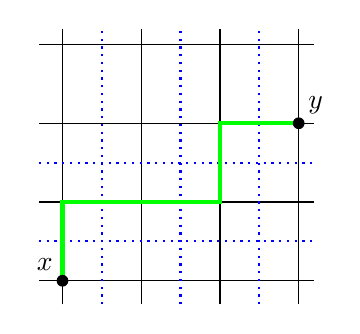
\begin{tikzpicture}[scale=1]
				\foreach \x in {1,...,4} {
					\draw (\x,0.7) -- (\x,4.2);
					\draw (0.7,\x) -- (4.2,\x);
				}
				
				\foreach \x in {1,2} {
					\draw [color=blue,dotted,thick] (0.7,\x+.5) -- (4.2,\x +.5);
					\draw [color=blue,dotted,thick] (\x+.5,0.7) -- (\x+.5,4.2);
				}
				
				\draw [color=blue,dotted,thick] (3.5,0.7) -- (3.5,4.2);
				
				\draw [color=green,ultra thick] (1,1) -- (1,2) -- (3,2) -- (3,3) -- (4,3);
				
				\draw (1,1) node[fill,circle,inner sep=1.5pt]{};
				\draw (4,3) node[fill,circle,inner sep=1.5pt]{};
				\draw (1,1) node[anchor=south east]{$x$};
				\draw (4,3) node[anchor=south west]{$y$};
			\end{tikzpicture} \hspace{2cm}
			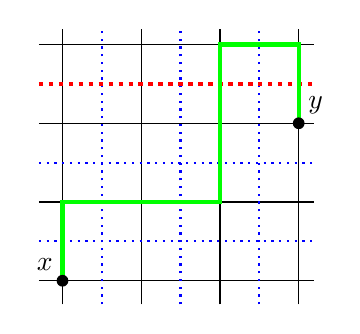
\begin{tikzpicture}[scale=1]
				\foreach \x in {1,...,4} {
					\draw (\x,0.7) -- (\x,4.2);
					\draw (0.7,\x) -- (4.2,\x);
				}
				
				\foreach \x in {1,2} {
					\draw [color=blue,dotted,thick] (0.7,\x+.5) -- (4.2,\x +.5);
					\draw [color=blue,dotted,thick] (\x+.5,0.7) -- (\x+.5,4.2);
				}
				
				\draw [color=blue,dotted,thick] (3.5,0.7) -- (3.5,4.2);
				\draw [color=red,dotted,ultra thick] (.7,3.5) -- (4.2,3.5);
				
				\draw [color=green,ultra thick] (1,1) -- (1,2) -- (3,2) -- (3,4) -- (4,4) -- (4,3);
				
				\draw (1,1) node[fill,circle,inner sep=1.5pt]{};
				\draw (4,3) node[fill,circle,inner sep=1.5pt]{};
				\draw (1,1) node[anchor=south east]{$x$};
				\draw (4,3) node[anchor=south west]{$y$};
			\end{tikzpicture}
			\caption*{Links: Ein kürzester Weg zwischen $x$ und $y$. Rechts: Ein längerer Weg, der eine Hyperebene zwei Mal schneidet.}
		\end{figure}
		Diese Hyperebenen liefern genau diejenigen Halbräume von $X$ die entweder $x$ oder $y$ enthalten ($x$ und $y$ liegen nicht auf einer Hyperebene, da diese die Kanten nur in ihren Mittelpunkten schneiden und nicht in Punkten aus $X^{(0)}$). Jede Hyperebene liefert zwei Halbräume: Einen Halbraum $U^+ \subseteq X$ mit $x \in U^+, y \notin U^+$, und einen Halbraum $U^- \subseteq X$ mit $x \notin U^-, y \in U^-$.
		\newpage
		Somit stimmt die Anzahl der Hyperebenen zwischen $x$ und $y$ überein mit der Anzahl der Halbräume von $X$, die $x$ enthalten und $y$ nicht. Zusammengefasst:
		\begin{equation}
		\begin{aligned}
			D(x,y) &= \inf \{ \ell(\sigma) : \sigma \text{ ist Weg von } x \text{ nach } y \text{ in } X^{(1)}\} \\
			&= \#\{H \subseteq X : H \text{ ist Hyperebene zwischen } x \text{ und } y\} \\
			&= \#\{U \subseteq X \text{ Halbraum} : x \in U, y \notin U \} \\
			&= \sum_{\substack{U \subseteq X \\ \text{Halbraum}}} \underbrace{\chi_U(x) \cdot (1- \chi_U(y))}_{= 1 \Leftrightarrow x \in U \wedge y \notin U}
		\end{aligned}
		\end{equation}
		\item Zu zeigen sind die Eigenschaften (1), (2) und (3) aus Definition \ref{def_cnk}. \\
		(1) und (2) sind klarerweise erfüllt, da $D$ eine Metrik ist. Sei also $V:= \{x_1, \dots, x_n\} \subseteq X^{(0)}$ endlich sowie $\lambda_1, \dots, \lambda_n \in \RR$ mit $\sum_{i=1}^{n} \lambda_i = 0$. Dann ist
		\[ \sum\limits_{1 \leq i,j \leq n} \lambda_i \lambda_j D(x_i,x_j) = \sum\limits_{i=1}^{n} \sum\limits_{j=1}^{n} \lambda_i \lambda_j \sum\limits_{U} \chi_U (x_i) (1-\chi_U (x_j))\]
		Da für jedes Paar $(x_i,x_j) \in V \times V$ höchstens endlich viele Hyperebenen zwischen $x_i$ und $x_j$ verlaufen, existieren insgesamt nur endlich viele Halbräume $U \subseteq X$, für die der Ausdruck\linebreak $\chi_U(x_i) \cdot (1-\chi_U(x_j))$ in der hinteren Summe nicht verschwindet. Insbesondere ist die hintere Summe endlich. Bezeichnen wir jene Halbräume mit $U_1, \dots, U_m$, ermöglicht dies folgende Umformungen:
		\begin{equation}
		\begin{aligned}
			\ &\sum\limits_{i=1}^{n} \sum\limits_{j=1}^{n} \lambda_i \lambda_j \sum\limits_{k=1}^m \chi_{U_k} (x_i) - \sum\limits_{i=1}^{n} \sum\limits_{j=1}^{n} \lambda_i \lambda_j \sum\limits_{k=1}^m \chi_{U_k} (x_i) \cdot \chi_{U_k} (x_j) \\
			= \  &\underbrace{\sum\limits_{j=1}^{n} \lambda_j}_{=0} \sum\limits_{i=1}^{n} \lambda_i \sum\limits_{k=1}^m \chi_{U_k} (x_i) - \sum\limits_{k=1}^m \sum\limits_{i=1}^{n} \lambda_i \chi_{U_k}(x_i) \sum\limits_{j=1}^{n} \lambda_j \chi_{U_k} (x_j) \\
			= \ &0 - \sum\limits_{k=1}^m \enbrace*{\sum\limits_{i=1}^n \lambda_i \chi_{U_k} (x_i)}^2 
			\leq 0
		\end{aligned}
		\end{equation}
		\item Wie in Definition \ref{def_D} bemerkt, stimmt die simpliziale Metrik $D$ auf $X^{(0)}$ mit der Längenmetrik $d_{X^{(1)}}$ von $X^{(1)}$ eingeschränkt auf $X^{(0)}$ überein. Da $(X^{(1)},d_{X^{(1)}})$ ein kubischer Komplex ist, vermittelt $\Phi$ auch eine simpliziale (und damit isometrische) Wirkung $\widetilde{\Phi}$ auf $X^{(1)}$ vermöge $\widetilde{\Phi}(g) := \Phi(g) \big|_{X^{(1)}}$, das heißt für alle $x,y \in X^{(0)} \subseteq X^{(1)}$ und $g \in G$ gilt
		\[ D(\Phi(g)(x),\Phi(g)(y)) = d_{X^{(1)}}(\widetilde{\Phi}(g)(x),\widetilde{\Phi}(g)(y)) = d_{X^{(1)}}(x,y) = D(x,y) \qed \]		
	\end{enumerate}
	
\begin{satz2}[Niblo, Reeves]
	Sei $X$ ein vollständiger $\cat$ kubischer Komplex und $G$ eine endlich erzeugte Gruppe, die die Kazhdan-Eigenschaft $\prT$ erfüllt. Dann hat jede simpliziale Wirkung von $G$ auf $X$ einen globalen Fixpunkt. Mit anderen Worten:
	\[ G \text{ hat Eigenschaft } \prT \quad \Rightarrow \quad G \text{ hat Eigenschaft } \FSC \]
\end{satz2}

\minisec{Bemerkung}
	Aus dem Theorem folgt unmittelbar, dass jede Gruppe mit Kazhdan-Eigenschaft $\prT$ auch die Serre-Eigenschaft $\operatorname{FA}$ erfüllt, da jeder Baum ein vollständiger $\cat$ kubischer Komplex ist.

\minisec{Beweis des Theorems}
	Sei $\Phi\colon G \rightarrow \Isom(X)$ eine beliebige simpliziale Wirkung von $G$ auf $X$. Dann ist $\Phi\big|_{X^{(0)}}\colon G \rightarrow \Isom(X^{(0)})$ eine simpliziale Wirkung auf dem $0$-Skelett von $X$. Wir fixieren ein $v \in X^{(0)}$ beliebig und betrachten die Abbildung
	\begin{equation}
	\begin{aligned}
		f_v\colon G \times G &\longrightarrow \RR \\
		(g,h) &\longmapsto D(\Phi(g)(v),\Phi(h)(v))
	\end{aligned}
	\end{equation}
	Wir zeigen, dass $f_v$ ein bedingt negativ definiter Kern auf $G$ ist. Die Eigenschaften (1), (2) und (3) sind klarerweise erfüllt, da $D$ ein bedingt negativ definiter Kern ist. Die Linksinvarianz von $f_v$ folgt aus der Invarianz von $D$: Für beliebige $g,h,k \in G$ gilt:
	\begin{equation}
	\begin{aligned}
		f_v(gh,gk) &= D(\Phi(gh)(v),\Phi(gk)(v)) \\
		&= D(\Phi(g)(\Phi(h)(v)),\Phi(g)(\Phi(k)(v))) \\
		&= D(\Phi(h)(v),\Phi(k)(v)) \\
		&= f_v(h,k)
	\end{aligned}
	\end{equation}
	Die Gruppe $G$ hat Eigenschaft $\prT$, also ist $f_v$ beschränkt, das heißt die Menge\linebreak $f_v(G \times G) = D(\Phi(G)(v) \times \Phi(G)(v))$ ist beschränkt in $\RR$. Damit ist der Orbit $\Phi(G)(v)$ von $v$ beschränkt bezüglich $D$ und wegen $d \leq D$ (vgl. Bemerkung nach Def. \ref{def_D}) auch bezüglich $d$. Nach Voraussetzung ist $(X,d)$ vollständig und $\cat$. Mit dem Fixpunktsatz von Bruhat-Tits folgt also die Existenz eines Fixpunktes. \qed
